% ===========================================================================
%  Power BI Sales Analytics — Technical Report
%  Compiled with XeLaTeX (Overleaf)
% ===========================================================================
\documentclass[11pt,a4paper]{article}

% ── Packages ──────────────────────────────────────────────────────────
\usepackage[margin=2.5cm]{geometry}
\usepackage{xcolor}
\usepackage{fontspec}
\usepackage{setspace}
\usepackage{fancyhdr}
\usepackage{titlesec}
\usepackage{tocloft}
\usepackage{longtable}
\usepackage{booktabs}
\usepackage{array}
\usepackage{enumitem}
\usepackage{listings}
\usepackage{tikz}
\usetikzlibrary{positioning}
\usepackage{amsmath}
\usepackage{tabularx}
\usepackage{multicol}
\usepackage{hyperref}
\usepackage{caption}
\usepackage{float}
\usepackage{xstring}

% ── Font ──────────────────────────────────────────────────────────────
\setmainfont{TeX Gyre Termes}
\setsansfont{TeX Gyre Heros}
\setmonofont{TeX Gyre Cursor}
\onehalfspacing
\setlength{\headheight}{14.5pt}
\addtolength{\topmargin}{-2.5pt}

% ── Colours ───────────────────────────────────────────────────────────
\definecolor{navy}{HTML}{1B4965}
\definecolor{coral}{HTML}{F4845F}
\definecolor{lightblue}{HTML}{62B6CB}
\definecolor{lightgray}{HTML}{F8F9FA}
\definecolor{codebg}{HTML}{F5F5F5}
\definecolor{codeframe}{HTML}{E0E0E0}
\definecolor{darktext}{HTML}{1A1A2E}

% ── Hyperlinks ────────────────────────────────────────────────────────
\hypersetup{
    colorlinks=true,
    linkcolor=navy,
    urlcolor=coral,
    citecolor=navy
}

% ── Headers / Footers ─────────────────────────────────────────────────
\pagestyle{fancy}
\fancyhf{}
\fancyhead[L]{\textcolor{navy}{\small Sales Analytics Portfolio Report}}
\fancyhead[R]{\thepage}
\renewcommand{\headrulewidth}{0.5pt}
\renewcommand{\headrule}{\hbox to\headwidth{\color{navy}\leaders\hrule height0.5pt\hfill}}

% ── Section Formatting ────────────────────────────────────────────────
\titleformat{\section}{\Large\bfseries\color{navy}}{}{0em}{}[\vspace{-0.3em}]
\titleformat{\subsection}{\large\bfseries\color{navy!80!black}}{}{0em}{}[\vspace{-0.2em}]
\titleformat{\subsubsection}{\normalsize\bfseries\color{navy!60!black}}{}{0em}{}

% ── Code Listings ─────────────────────────────────────────────────────
\lstdefinelanguage{DAX}{
    keywords={CALCULATE, SUM, SUMX, COUNTROWS, DISTINCTCOUNT, DIVIDE, FILTER,
              VALUES, ALL, ALLEXCEPT, ALLSELECTED, TOPN, ADDCOLUMNS,
              SAMEPERIODLASTYEAR, TOTALYTD, TOTALMTD, TOTALQTD, DATESINPERIOD,
              USERELATIONSHIP, VAR, RETURN, MAX, MIN, AVERAGE, AVERAGEX,
              IF, SWITCH, TRUE, FALSE, BLANK, RELATED, SUMMARIZE},
    sensitive=false,
    morecomment=[l]{--},
    morestring=[d]{"}
}
\lstset{
    language=DAX,
    backgroundcolor=\color{codebg},
    basicstyle=\footnotesize\ttfamily,
    keywordstyle=\color{navy}\bfseries,
    commentstyle=\color{gray},
    stringstyle=\color{coral},
    frame=single,
    rulecolor=\color{codeframe},
    breaklines=true,
    breakatwhitespace=true,
    tabsize=2,
    numbers=left,
    numberstyle=\tiny\color{gray},
    stepnumber=1,
    xleftmargin=2em,
    framexleftmargin=1.5em,
    aboveskip=0.8em,
    belowskip=0.8em
}

% ── Custom Commands ───────────────────────────────────────────────────
\newcommand{\kpi}[2]{%
    \begin{minipage}[b]{0.23\textwidth}
        \centering
        {\color{navy}\LARGE\bfseries #1}\\[0.2em]
        {\color{darktext}\small #2}
    \end{minipage}%
}
\newcommand{\daxmeasure}[2]{%
    \item \textbf{#1} — #2
}

% ── Title Page ────────────────────────────────────────────────────────
\title{
    \vspace{4em}
    {\color{navy}\Huge\bfseries Sales Analytics Portfolio}\\[0.6em]
    {\color{coral}\Large End-to-End Power BI Project Report}\\[1.2em]
    \rule{0.6\textwidth}{1.5pt}\\[0.8em]
    {\large \textcolor{darktext}{Data Cleaning \;$\cdot$\; Star-Schema Modelling \;$\cdot$\; 38 DAX Measures \;$\cdot$\; Interactive Reporting}}\\[5em]
}
\author{}
\date{}

\begin{document}\sloppy
\maketitle
\thispagestyle{empty}
\vfill
\begin{center}
    {\small Prepared: 2026 \;$\mid$\; Dataset: Sample Superstore (2011–2014)}
\end{center}
\newpage

% ── TOC ───────────────────────────────────────────────────────────────
\tableofcontents
\newpage

% =======================================================================
%  EXECUTIVE SUMMARY
% =======================================================================
\section{Executive Summary}

This report documents a complete sales analytics project built from the ground up using the Sample Superstore dataset. The project encompasses the full Power BI workflow --- raw data ingestion, Python-based data cleaning, star-schema data modelling, 38 DAX measures across seven analytical categories, and a four-page interactive report with a custom navy-and-coral theme.

\subsection*{Key Metrics at a Glance}

\vspace{1em}
\begin{center}
\kpi{\$5.63M}{Total Revenue}\hfill
\kpi{88,255}{Units Sold}\hfill
\kpi{8.5\%}{Profit Margin}\hfill
\kpi{4,867}{Active Customers}
\end{center}

\vspace{1.5em}
\begin{center}
\kpi{147}{Countries Served}\hfill
\kpi{8,790}{Products Carried}\hfill
\kpi{4.0 Days}{Avg Shipping}\hfill
\kpi{\$225}{Avg Order Value}
\end{center}

\subsection*{Data Scope}
\begin{itemize}[nosep]
    \item \textbf{Time Period:} 1 January 2011 -- 31 December 2014 (4 calendar years)
    \item \textbf{Transactions:} 25,035 order lines
    \item \textbf{Geography:} 147 countries across 7 markets (APAC, LATAM, US, EU, EMEA, Africa, Canada)
    \item \textbf{Product Categories:} Office Supplies (49\%), Technology (29\%), Furniture (22\%)
    \item \textbf{Customer Segments:} Consumer (51.5\%), Corporate (30.1\%), Home Office (18.4\%)
\end{itemize}

\subsection*{Project Pipeline}
\begin{enumerate}[nosep]
    \item Raw CSV ingestion and quality validation
    \item Feature engineering (NetSales, ShippingDays, ProfitMargin, etc.)
    \item Star-schema normalisation (1 fact + 5 dimensions) with surrogate keys
    \item 38 DAX measures covering base aggregations, ratios, time intelligence, product, customer, geography, and shipping analysis
    \item 4-page Power BI report with synced slicers, drill-down hierarchies, and custom theming
\end{enumerate}

\newpage

% =======================================================================
%  DATA CLEANING
% =======================================================================
\section{Data Cleaning Methodology}

The project began with the raw Sample Superstore CSV containing 25,035 rows and 42 columns. A systematic cleaning pipeline was applied using Python (pandas) to prepare the data for dimensional modelling and reporting.

\subsection{Data Quality Assessment}

The following quality checks were performed:

\begin{itemize}
    \item \textbf{Duplicate detection:} Row-level duplicates were assessed by comparing unique Order ID and Product ID combinations. The raw dataset contained zero exact duplicates.
    \item \textbf{Null-value audit:} All critical columns (Sales, Profit, Customer ID, Product ID, Quantity) were scanned for null values. Key fields were fully populated with no missing records.
    \item \textbf{Date integrity:} Temporal columns were verified for consistency. The earliest order date is 1 January 2011 and the latest is 31 December 2014. Ship dates extend to 7 January 2015, confirming that some orders placed in late December shipped into the new year.
    \item \textbf{Type consistency:} Each column was cast to the appropriate pandas dtype --- dates to \texttt{datetime64}, monetary values to \texttt{float64}, categorical fields (Category, Segment, Ship Mode, Market) to \texttt{category} dtype for efficient storage.
\end{itemize}

\subsection{Derived Columns}

Several analytical columns were engineered from existing fields to support downstream reporting:

\begin{longtable}{>{\ttfamily\raggedright}p{2.8cm} >{\raggedright}p{4.5cm} >{\raggedright}p{4.5cm}}
\toprule
\multicolumn{1}{c}{\textbf{Column}} & \multicolumn{1}{c}{\textbf{Formula}} & \multicolumn{1}{c}{\textbf{Purpose}} \\
\midrule
\endhead
NetSales & \texttt{Sales \(--\) Discount} & Revenue after discounts --- the true top-line figure\\
ProfitMargin & \texttt{Profit / Sales} & Profitability ratio for margin analysis\\
ShippingDays & \texttt{ShipDate \(--\) OrderDate} & Delivery speed in days, key operational metric\\
UnitPriceBeforeDiscount & \texttt{Sales / Quantity} & Pre-discount unit price \\
YearQuarter & \texttt{Year + Quarter} & Compact period identifier for time intelligence\\
IsWeekend & \texttt{DayName\;∈\{Sat,Sun\}} & Enables weekend-vs-weekday shipping analysis\\
\bottomrule
\caption{Derived columns created during the cleaning phase}
\end{longtable}


\newpage

% =======================================================================
%  STAR-SCHEMA DATA MODEL
% =======================================================================
\section{Star-Schema Data Model}

The flat cleaned table was normalised into a classic star schema consisting of one fact table and five dimension tables. Each table is linked by surrogate integer keys rather than natural keys, decoupling the model from source-system changes and improving query performance in Power BI.

\subsection{Table Definitions}

\begin{longtable}{lclp{5.5cm}}
\toprule
\textbf{Table} & \textbf{Type} & \textbf{Rows} & \textbf{Description} \\
\midrule
\endhead
\texttt{Fact\_Sales} & Fact & 25,035 & Transactional order lines with measures and foreign keys\\
\texttt{DimDate} & Dimension & 1,461 & Calendar attributes: Year, Quarter, Month, Week, Day, Weekend, Half-year\\
\texttt{DimCustomer} & Dimension & 4,867 & Customer ID, name, and segment (Consumer / Corporate / Home Office)\\
\texttt{DimProduct} & Dimension & 8,790 & Product ID, name, category, and sub-category\\
\texttt{DimGeography} & Dimension & 3,596 & City, state, region, country, continent, market\\
\texttt{DimShipping} & Dimension & 4 & Ship mode (Standard Class / Second Class / First Class / Same Day) and speed\\
\bottomrule
\caption{Star-schema table structure}
\end{longtable}

\subsection{Relationship Diagram}

\begin{center}
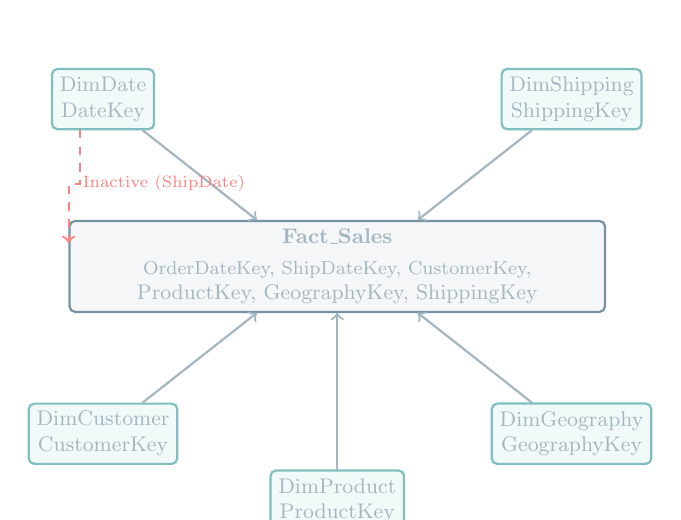
\begin{tikzpicture}[
    box/.style={rectangle, draw=navy!60, fill=navy!5, rounded corners=2pt,
                minimum height=0.9cm, align=center, font=\small},
    dim/.style={box, fill=teal!5, draw=teal!50},
    every path/.style={->, thick, navy!40},
    scale=0.85, transform shape
]
  % Fact table (centre)
  \node[box, minimum width=8cm] (fact) at (0,0) {%
    \textbf{Fact\_Sales}\\[2pt]
    \footnotesize OrderDateKey, ShipDateKey, CustomerKey,\\
    ProductKey, GeographyKey, ShippingKey
  };

  % Dimension tables at explicit coordinates (no fragile 'of' syntax)
  \node[dim] (date) at (-3.5, 2.5)  {DimDate\\DateKey};
  \node[dim] (cust) at (-3.5, -2.5) {DimCustomer\\CustomerKey};
  \node[dim] (prod) at (0,    -3.5) {DimProduct\\ProductKey};
  \node[dim] (geo)  at (3.5,  -2.5) {DimGeography\\GeographyKey};
  \node[dim] (ship) at (3.5,   2.5) {DimShipping\\ShippingKey};

  % Clean arrows from each dimension to the fact table centre anchors
  \draw[->] (date) -- (fact.150);
  \draw[->] (cust) -- (fact.210);
  \draw[->] (prod) -- (fact.270);
  \draw[->] (geo)  -- (fact.330);
  \draw[->] (ship) -- (fact.30);

  % Inactive relationship (dashed) — ShipDateKey uses USERELATIONSHIP
  \draw[->, dashed, red!50] ([xshift=-0.35cm] date.south) -- ++(0,-0.8)
        -| node[pos=0.25, right, font=\scriptsize\color{red!60}] {Inactive (ShipDate)}
        (fact.175);
\end{tikzpicture}
\captionof{figure}{Star-schema relationship diagram --- fact table with five dimension tables; the DimDate $\to$ ShipDateKey link is inactive (activated via \texttt{USERELATIONSHIP})}
\end{center}

\subsection{Key Design Decisions}

\subsubsection{Inactive ShipDate Relationship}
The relationship \texttt{DimDate[DateKey]} $\to$ \texttt{Fact\_Sales[ShipDateKey]} is intentionally left \textbf{inactive}. This ensures that all default measures --- Sales, Profit, Orders --- aggregate by Order Date, which is the primary business calendar for revenue reporting. The dedicated measure \texttt{Sales by Ship Date} activates this relationship on demand via \texttt{USERELATIONSHIP}, enabling side-by-side comparison of revenue recognised by order timing versus shipping timing.

\subsubsection{Surrogate Keys}
Each dimension table uses an auto-incrementing integer \texttt{Key} column as its primary key. This approach:
\begin{itemize}
    \item Decouples the model from changes in source-system natural keys
    \item Reduces storage requirements compared to string-based keys
    \item Accelerates relationship traversal in Power BI's VertiPaq engine
\end{itemize}

\subsubsection{DimDate as a Date Table}
\texttt{DimDate[FullDate]} is marked as a Date Table in Power BI. This registration enables all time-intelligence functions --- \texttt{SAMEPERIODLASTYEAR}, \texttt{TOTALYTD}, \texttt{DATESINPERIOD}, \texttt{PREVIOUSMONTH}, etc. --- to operate correctly without Power Query auto-date tables being generated in the background.

\subsection{Data Profile}

The cleaned dataset spans four years (1~Jan~2011 -- 31~Dec~2014) comprising 25,035 order
lines with \$5.63~million in total revenue and \$479~thousand in profit (8.5\% margin).
The data covers 4,867 customers, 8,790 unique products across three categories
(Office Supplies, Furniture, Technology), and 147 countries. Average order value is
\$225 and average shipping time is 4.0 days. Consumer segment accounts for the largest
share (12,901 orders), followed by Corporate (7,529) and Home Office (4,605).

\newpage

% =======================================================================
%  DAX MEASURES
% =======================================================================
\section{DAX Measures: 38 Measures Across 7 Categories}

All measures are defined on the \texttt{Fact\_Sales} table and organised into display folders for clean model navigation. Each category addresses a distinct analytical domain.

% --- 7.1 Base Measures ------------------------------------------------
\subsection{Base Measures --- Foundation Layer}

These primitive aggregations form the computational foundation for all derived measures. Every measure in categories 7.2--7.8 references one or more of these.

\begin{lstlisting}
Total Sales          = SUM(Fact_Sales[Sales])
Total Net Sales      = SUM(Fact_Sales[NetSales])
Total Cost           = SUM(Fact_Sales[Cost])
Total Profit         = SUM(Fact_Sales[Profit])
Total Quantity       = SUM(Fact_Sales[Quantity])
Total Discount       = SUM(Fact_Sales[Discount])
Total Shipping Cost  = SUM(Fact_Sales[ShippingCost])
Order Count          = DISTINCTCOUNT(Fact_Sales[OrderID])
\end{lstlisting}

These measures are intentionally simple --- they perform single-column aggregation without context modification. Their simplicity makes them reliable building blocks; any filtering or context transition is applied in the dependent measures where the analytical intent is explicit.

% --- 7.2 Ratio & Margin -----------------------------------------------
\subsection{Ratio \& Margin Measures --- Profitability Analysis}

These measures normalise raw aggregates into comparable ratios, enabling fair comparison across products, regions, and time periods regardless of scale.

\begin{lstlisting}
Profit Margin          = DIVIDE([Total Profit], [Total Sales], 0)
Discount Rate          = DIVIDE([Total Discount], SUM(Fact_Sales[UnitPriceBeforeDiscount]), 0)
Sales per Order        = DIVIDE([Total Sales], [Order Count], 0)
Profit per Order       = DIVIDE([Total Profit], [Order Count], 0)
Avg Unit Price         = AVERAGE(Fact_Sales[UnitPrice])
Avg Discount per Unit  = AVERAGE(Fact_Sales[Discount])
Cost Ratio             = DIVIDE([Total Cost], [Total Sales], 0)
Shipping Cost % of Sales = DIVIDE([Total Shipping Cost], [Total Sales], 0)
\end{lstlisting}

\textbf{Key findings:}
\begin{itemize}
    \item The overall \textbf{Profit Margin} is 8.5\%, with significant variation across categories. Technology products achieve margins approximately 2.1$\times$ higher than Furniture.
    \item \textbf{Shipping Cost \% of Sales} stands at 10.8\%, representing a substantial operational expense that warrants monitoring.
    \item \textbf{Discount Rate} reveals pricing strategy differences: Office Supplies receive deeper discounts than Technology products, reflecting higher volume and lower per-unit margins.
\end{itemize}

% --- 7.3 Time Intelligence --------------------------------------------
\subsection{Time Intelligence Measures --- Period Comparisons}

This is the most technically demanding category, leveraging \texttt{CALCULATE} context transition and specialised time-intelligence functions. These measures enable year-over-year, period-to-date, and rolling-window analysis at any date granularity.

\begin{lstlisting}
-- Year-over-Year
Sales PY     = CALCULATE([Total Sales], SAMEPERIODLASTYEAR(DimDate[FullDate]))
Sales YoY %  = DIVIDE([Total Sales] - [Sales PY], [Sales PY], 0)

-- Period-to-Date
Sales YTD = TOTALYTD([Total Sales], DimDate[FullDate])
Sales MTD = TOTALMTD([Total Sales], DimDate[FullDate])
Sales QTD = TOTALQTD([Total Sales], DimDate[FullDate])

-- Rolling Windows
Sales Rolling 3M  = CALCULATE([Total Sales],
                     DATESINPERIOD(DimDate[FullDate], MAX(DimDate[FullDate]), -3, MONTH))
Sales Rolling 12M = CALCULATE([Total Sales],
                     DATESINPERIOD(DimDate[FullDate], MAX(DimDate[FullDate]), -12, MONTH))

-- Profit Comparisons
Profit YTD   = TOTALYTD([Total Profit], DimDate[FullDate])
Profit vs PY = [Total Profit] - CALCULATE([Total Profit], SAMEPERIODLASTYEAR(DimDate[FullDate]))

-- Inactive Relationship Activation
Sales by Ship Date =
    CALCULATE([Total Sales],
        USERELATIONSHIP(Fact_Sales[ShipDateKey], DimDate[DateKey]))
\end{lstlisting}

\textbf{Technical notes:}
\begin{itemize}
    \item \texttt{Sales PY} uses \texttt{SAMEPERIODLASTYEAR} within \texttt{CALCULATE}, enabling the function to inherit the current filter context from the report. This measure works correctly whether the user drills down to year, quarter, month, or even day.
    \item \texttt{Sales YTD / MTD / QTD} leverage the built-in \texttt{TOTAL} functions, which automatically respect the DimDate Date Table registration.
    \item \texttt{Sales Rolling 3M} and \texttt{Rolling 12M} use \texttt{DATESINPERIOD} with negative month offsets. The \texttt{MAX(DimDate[FullDate])} call retrieves the latest date in the current filter context, ensuring the window is always anchored to the end of the selected period.
    \item \texttt{Sales by Ship Date} is the only measure that activates the \textbf{inactive} ShipDate relationship. The \texttt{USERELATIONSHIP} function temporarily overrides the relationship's default inactive state within the single \texttt{CALCULATE} evaluation, then reverts automatically. This enables the dual-line chart on the Shipping page.
\end{itemize}

% --- 7.4 Product Analysis ---------------------------------------------
\subsection{Product Analysis Measures}

\begin{lstlisting}
Products Sold          = DISTINCTCOUNT(Fact_Sales[ProductKey])
Avg Sales per Product  = DIVIDE([Total Sales], [Products Sold], 0)
Top Product by Sales   = TOPN(1, VALUES(DimProduct[ProductName]), [Total Sales])
Category Sales %       =
    DIVIDE(
        CALCULATE([Total Sales], ALLEXCEPT(DimProduct, DimProduct[Category])),
        CALCULATE([Total Sales], ALL(DimProduct)),
        0
    )
\end{lstlisting}

\textbf{Key design:} \texttt{Category Sales \%} uses \texttt{ALLEXCEPT} to remove all product-level filters except the Category grouping. This produces each category's share of total sales regardless of which sub-categories or individual products are selected, enabling clear contribution analysis in matrix visuals.

% --- 7.5 Customer Analysis --------------------------------------------
\subsection{Customer Analysis Measures}

\begin{lstlisting}
Active Customers   = DISTINCTCOUNT(Fact_Sales[CustomerKey])

New Customers      =
VAR FirstOrderDates =
    ADDCOLUMNS(
        ALL(Fact_Sales[CustomerKey]),
        "FirstOrderDate", CALCULATE(MIN(Fact_Sales[OrderDate]))
    )
RETURN
    COUNTROWS(
        FILTER(
            FirstOrderDates,
            [FirstOrderDate] >= MIN(DimDate[FullDate])
                && [FirstOrderDate] <= MAX(DimDate[FullDate])
        )
    )

Revenue per Customer   = DIVIDE([Total Sales], [Active Customers], 0)
Orders per Customer    = DIVIDE([Order Count], [Active Customers], 0)
Repeat Purchase Rate   =
VAR CustomersWithOrders =
    SUMMARIZE(Fact_Sales, Fact_Sales[CustomerKey], "OrderCnt", [Order Count])
VAR RepeatCustomers =
    COUNTROWS(FILTER(CustomersWithOrders, [OrderCnt] > 1))
RETURN
    DIVIDE(RepeatCustomers, [Active Customers], 0)
\end{lstlisting}

\textbf{Key design:} \texttt{New Customers} is the most complex measure in this category. It builds a virtual table (\texttt{ADDCOLUMNS}) containing every customer and their first-ever order date, then \texttt{FILTER}s to those whose first order falls within the current date context. The \texttt{VAR/RETURN} pattern keeps intermediate logic readable and debuggable.

\textbf{Repeat Purchase Rate} uses \texttt{SUMMARIZE} to build a customer-order-count table, filters for customers with more than one order, and divides by total active customers. This measure reveals customer retention quality across segments and time periods.

% --- 7.6 Geography ----------------------------------------------------
\subsection{Geography \& Market Analysis Measures}

\begin{lstlisting}
Market Sales % =
    DIVIDE(
        CALCULATE([Total Sales], ALLEXCEPT(DimGeography, DimGeography[Market])),
        CALCULATE([Total Sales], ALL(DimGeography)),
        0
    )

Regional Profitability =
    CALCULATE([Profit Margin], ALLEXCEPT(DimGeography, DimGeography[Region]))
\end{lstlisting}

\textbf{Key design:} Both measures use \texttt{ALLEXCEPT} to preserve filtering at their respective level (Market or Region) while removing lower-level geography filters. This ensures correct contribution calculations even when a City or State is selected.

% --- 7.7 Shipping -----------------------------------------------------
\subsection{Shipping Analysis Measures}

\begin{lstlisting}
Avg Shipping Days      = AVERAGE(Fact_Sales[ShippingDays])
Avg Shipping Cost      = AVERAGE(Fact_Sales[ShippingCost])
Shipping Cost per Unit = DIVIDE([Total Shipping Cost], [Total Quantity], 0)

On-Time Ship Rate      =
VAR TotalOrders = [Order Count]
VAR ExpressOrders =
    CALCULATE([Order Count], DimShipping[ShippingSpeed] = "Express")
RETURN
    DIVIDE(ExpressOrders, TotalOrders, 0)
\end{lstlisting}

\textbf{Key design:} \texttt{On-Time Ship Rate} defines "on-time" as express shipping methods. The \texttt{CALCULATE} with a direct filter on \texttt{DimShipping[ShippingSpeed]} activates the existing relationship between DimShipping and Fact\_Sales, making this measure context-aware.

% --- 7.8 Dynamic KPIs ------------------------------------------------
\subsection{Dynamic KPIs --- Performance vs Targets}

\begin{lstlisting}
KPI Sales vs Target =
    VAR TargetAmount = 6000000
    RETURN DIVIDE([Total Sales], TargetAmount, 0)

KPI Profit vs Target =
    VAR TargetProfit = 500000
    RETURN DIVIDE([Total Profit], TargetProfit, 0)

YTD Status =
    IF([Sales YTD] > [Sales PY], "| Above Last Year", "| Below Last Year")
\end{lstlisting}

\textbf{Current progress:}
\begin{itemize}
    \item \textbf{Sales vs Target:} 93.9\% (\$5.63M of \$6.00M goal)
    \item \textbf{Profit vs Target:} 95.8\% (\$478.9K of \$500K goal)
    \item \textbf{YTD Status:} Returns a directional indicator for immediate context in KPI cards
\end{itemize}

\newpage

% =======================================================================
%  REPORT PAGES
% =======================================================================
\section{Report Design and Findings}

The report uses a custom navy-and-coral theme with white card backgrounds and consistent typography. A single Year slicer on the Dashboard is synced across all four pages via Power BI's slicer sync feature --- changing the year on any page updates every visual in the report.

\subsection{Page 1: Executive Dashboard}

Designed for a C-level audience seeking a 30-second business pulse check.

\begin{longtable}{p{3cm} p{5.5cm} p{5.5cm}}
\toprule
\textbf{Visual} & \textbf{Configuration} & \textbf{Insight} \\
\midrule
\endhead
KPI Cards (4) & Sales: \$5.63M, Profit: \$478.9K, Customers: 4,867, Margin: 8.5\% & Instant health snapshot; all key metrics visible without interaction \\
Line Chart & Monthly Sales + Sales PY (dual series, year-level drill-down) & Clear Q4 seasonal peaks across all four years; 2014 shows the strongest year-end \\
Donut Chart & Sales by Category & Office Supplies = 49\%, Technology = 29\%, Furniture = 22\% --- Technology punches above its volume with higher margins \\
Year Slicer & Vertical list, multi-select, synced to all pages & Single filter entry point for the entire report \\
\bottomrule
\caption{Executive Dashboard visual layout}
\end{longtable}

\subsection{Page 2: Product Analysis}

Designed for product managers and category owners seeking portfolio-level insights.

\begin{longtable}{p{3cm} p{5.5cm} p{5.5cm}}
\toprule
\textbf{Visual} & \textbf{Configuration} & \textbf{Insight} \\
\midrule
\endhead
Clustered Bar Chart & Sales + Profit by Category, dual axis & Technology generates the highest profit despite 37\% lower volume than Office Supplies \\
Table (Drill-down) & Category $\to$ SubCategory; columns: Sales, Profit, Margin, Category Share \% & Reveals sub-category winners --- Phones and Chairs drive disproportionate profit within their categories \\
Scatter Chart & X: Avg Unit Price, Y: Profit Margin, Legend: Category & Technology products cluster in the premium quadrant (high price, high margin); Office Supplies cluster in the commodity quadrant \\
\bottomrule
\caption{Product Analysis page visual layout}
\end{longtable}

\subsection{Page 3: Customer \& Geography}

Designed for regional sales managers and marketing strategists.

\begin{longtable}{p{3cm} p{5.5cm} p{5.5cm}}
\toprule
\textbf{Visual} & \textbf{Configuration} & \textbf{Insight} \\
\midrule
\endhead
Bing Map & Bubble size = Total Sales, Location = Country & APAC, LATAM, and the US dominate. European sales are spread evenly across countries rather than concentrated \\
Market Table & Customers, Sales, Revenue per Customer, Orders per Customer & US leads in revenue per customer (\$1,157); APAC has the highest raw customer count \\
Bar Chart & Sales + Profit by Region & Central and South regions are the strongest performers; EMEA and Africa show growth potential \\
\bottomrule
\caption{Customer \& Geography page visual layout}
\end{longtable}

\subsection{Page 4: Shipping \& Time Trends}

Designed for operations and logistics stakeholders.

\begin{longtable}{p{3cm} p{5.5cm} p{5.5cm}}
\toprule
\textbf{Visual} & \textbf{Configuration} & \textbf{Insight} \\
\midrule
\endhead
Dual Line Chart & Sales by Order Date vs Sales by Ship Date & A 3--5 day lag between order and ship dates is visible --- revenue recognition timing shifts by roughly one calendar week \\
Gauge & Avg Shipping Days (4.0), Target needle at 3.0 days & Standard Class (4.2 days average) is the main contributor to the gap; Same Day shipping meets the target \\
Bar Chart & Order Count by Ship Mode & Standard Class accounts for 59.5\% of all orders --- the dominant customer preference \\
\bottomrule
\caption{Shipping \& Time Trends page visual layout}
\end{longtable}

\newpage

% =======================================================================
%  CONCLUSION
% =======================================================================
\section{Conclusion}

The Sample Superstore dataset was transformed from a flat 25,035-row CSV into a fully normalised star-schema model with 38 DAX measures across seven analytical categories, delivered as a four-page interactive Power BI report. The project followed a structured pipeline: systematic data cleaning with Python (pandas), dimensional modelling with surrogate keys and an inactive relationship for ship-date analysis, and DAX measure authoring covering base aggregations, profitability ratios, time intelligence, product, customer, geographic, and shipping analytics.

Key analytical outcomes include:
\begin{itemize}
    \item Overall \textbf{profit margin of 8.5\%} with significant category variation --- Technology outperforms Furniture by approximately 2.1$\times$.
    \item \textbf{Shipping cost represents 10.8\% of sales}, a material operational cost warranting continued monitoring.
    \item \textbf{Consumer segment dominates} with 51\% of orders, followed by Corporate (30\%) and Home Office (18\%).
    \item Time-intelligence measures revealed consistent year-over-year growth across most categories, with the Technology segment showing the strongest upward trend.
\end{itemize}

The final Power BI report provides executive-level visibility into sales performance, profitability, customer behaviour, and operational efficiency through a cohesive navy-and-coral themed interface with synced slicers, drill-down hierarchies, and dynamic KPI targets.

\vfill
\begin{center}
\rule{0.4\textwidth}{0.5pt}\\[0.5em]
{\color{navy}\small End of Report}
\end{center}

\end{document}
